\documentclass[a4paper, 12pt]{scrreprt}

\usepackage[utf8]{inputenc}

\usepackage[T1]{fontenc}
\usepackage{listings}
\usepackage{float}
\usepackage{longtable}
\usepackage{graphicx}
\usepackage{hyperref}
\usepackage{textcomp}
\usepackage{caption}
\usepackage{parskip}
\usepackage[onehalfspacing]{setspace}
\usepackage{chngcntr}
\usepackage{acronym}
\usepackage{fancyhdr}
\usepackage[table,xcdraw,pdftex]{xcolor}

\usepackage{jslistings}


\lstset{basicstyle=\footnotesize\ttfamily\small,
		breaklines=true,
		extendedchars=true,
		inputencoding=utf8,
		literate= 
			{ä}{{\"a}}1%
			{ö}{{\"o}}1%
			{ü}{{\"u}}1,%
}



\usepackage[
backend=biber,
sorting=none,
citestyle=authoryear,
natbib=true
]{biblatex}
\usepackage[ngerman]{babel}
\usepackage{enumitem}


\setlist[enumerate]{label*=\arabic*.}
\addbibresource{references.bib}
\hypersetup{
	colorlinks,
	linkcolor={black},
	citecolor={black},
	urlcolor={black}
}
\defbibfilter{bookInbook}{
	type=book or
	type=inbook
}
\graphicspath{ {./img/} }

\counterwithout{figure}{chapter}
\counterwithout{table}{chapter}

\newcommand\klammercite[1]{%
	(\citealt{#1})}

\parskip 1.75ex plus 0.5ex minus 0.5ex

\pagestyle{fancy}
\cfoot{\thepage}
\lhead[\leftmark]{}
\rhead[]{\leftmark}




\title{Platzhalter Titel}
\subtitle{}
\author{Lennart Ploog}
\publishers{IS Medieninformatik\\ Fakultät 4\\ Hochschule Bremen}

\makeatletter
\let\inserttitle\@title
\makeatother

\begin{document}
	\maketitle
	\newpage
	\tableofcontents
	\newpage
\section*{Abkürzungsverzeichnis}
	\begin{acronym}[Bash]
		\acro{CRDT}{Conflict-free replicated data type}
		\acro{SC}{Strong Consistency}
		\acro{SEC}{Strong Eventual Consistency}
		\acro{EC}{Eventual Consistency}
		\acro{CRTD}{Konfliktfeier Replizierter Datentyp}
		\acro{P2P}{Peer To Peer}
		\acro{HLC}{Hybrid Logical Clock}
		\acro{JSON}{JavaScript Object Notation}
		\acro{HTTP}{Hypertext Transfer Protocol}
		\acro{HTTPS}{Hypertext Transfer Protocol Secure}
		\acro{LWW}{Last-Writer-Wins}
		\acro{LWW-Register}{Last-Writer-Wins Register}
		\acro{G-Set}{Grow-Only Set}
	\end{acronym}
\chapter{Abstract}
TODO: Acronyms, Figures
\chapter{Einleitung}\label{sec:Einleitung}
\section{Problemfeld}\label{sec:Problemfeld}

Ob auf Reisen, im Supermarkt oder im Fahrstuhl -- Situationen, in denen mobile Endgeräte keine stabile Internetverbindung haben, kommen im Alltag häufiger vor als gewünscht. In vielen Entwicklungsländern und auch in ländlichen Gegenden entwickelter Industriestaaten fehlt dafür gar die komplette Infrastruktur. Im Laufe der letzten Jahre eröffneten Innovationen im Bereich der Browser-Technologien, allen voran der Service-Worker, neue Möglichkeiten für die Webentwicklung, insbesondere für sogenannte Offline-First Anwendungen. Als Offline-First Applikationen werden Webanwendungen bezeichnet, die ihre Funktionalität so weit es geht behalten, wenn die Verbindung zum Internet getrennt ist.

Eine der Kernherausforderungen der Entwicklung von Offline-First Applikationen ist die Synchronisation von Daten. Werden offline Änderungen vorgenommen, sollen diese nicht verloren gehen. Hat sich der Zustand der Applikation, beispielsweise durch Modifikationen eines anderen Nutzers, in der Zwischenzeit jedoch geändert, müssen beide Änderungen zusammengebracht, also synchronisiert werden. Der Prozess der Synchronisation ist oft aufwendig, denn zum Einen muss ermittelt werden, wo sich beide Replikationen unterscheiden und zum Anderen muss vermieden werden, dass die Änderungen sich in die Quere kommen. 

Gängige Lösungen zu einer solchen Zusammenführung von Daten umfassen die Nutzung bestimmter Datenbanken-Technologien. Dazu gehören Datenbanken mit implementierter Synchronisation wie CloudDB oder auch Backend-as-a-Service Produkte wie Firebase oder IBM Cloudant, welche ebenfalls eine solche Funktionalität anbieten. Um zu Vermeiden, die Applikation mit suboptimalen Datenbanken-Technologien umsetzen zu müssen, verzichten viele Applikationen bei Konflikten auf eine Synchronisation und einer der beiden Nutzer verliert seine vollbrachte Arbeit.

\section{Ziel der Arbeit} 

Ziel dieser Arbeit ist es, eine Lösung zur Synchronisation von Daten in Offline-First Anwendungen mit Hilfe von konfliktfreien replizierten Datentypen (CRDTs) umzusetzen. Der Einsatz von CRDTs ermöglicht, dass Daten in einem verteilten System in beliebiger Reihenfolge ausgetauscht werden können und dennoch zum gleichen Zustand aller Replikationen führen. Durch die Implementierung einer Datenstruktur, welche auf CRDTs aufbaut, kann der Prozess der Synchronisierung somit vermieden werden. Diese Lösung soll unabhängig von der gewählten Datenbank sein.

So ergeben sich folgende Forschungsfragen:

\begin{itemize}
	\item Wie können CRDTs in Offline-First Applikationen verwendet werden?
	\item Welche CRDTs bieten sich zur Umsetzung von Offline-First Applikationen an und wie werden diese in die Datenbanken (Client und Server) implementiert?
	\item Welche Vor- und Nachteile bietet die Nutzung von CRDTs im Vergleich zu anderen Optionen zur Synchronisierung von Daten in Offline-First Applikationen.
\end{itemize}

\section{Vorgehen}
Es gibt verschiedene Möglichkeiten, wie CRDTs in Webapplikationen eingesetzt werden können. Bevor die Implementation der Datenstruktur im hier entwickelten Prototypen beginnen kann, muss ermittelt werden, welche CRDTs sich am besten für die Daten des Prototypen eignen. Um dies herauszufinden, eignet sich die Recherche in den im Abschnitt Verwandte Arbeiten erwähnten Publikationen. Darüber hinaus lohnt es sich an dieser Stelle auch in Erfahrung zu bringen, welche CRDTs bis heute in fertigen Applikationen verwendet wurden. Auch Literatur zum Austausch von Daten in Applikationen zu kollaborativem Editieren zu \ac{P2P} Netzwerken bietet sich zur Recherche an, denn in diesen Bereichen sind CRDTs schon weiter verbreitet als in anderen Anwendungsgebieten.

Damit der Prototyp als praxisnahes Beispiel dienen kann, sollte auch der Stand der Technik im Themenbereich der Offline-First Anwendungen ermittelt werden. Um einzuordnen, auf welcher Ebene der Architektur der Applikation sich die umzusetzende Funktionalität zur Zusammenführung der Daten am besten einbauen lässt, lohnt sich auch ein Blick auf bestehende Lösungen, welche die Synchronisation nicht direkt auf der Datenbankebene durchführen, sondern zwischen Applikation und Datenbank.

\subsection{Prototyp}
Platzhalter, genauer nach Fertigstellung des Prototypen
Als Prototyp wird ein Online-Kochbuch mit folgenden Funktionen umgesetzt:
\begin{itemize}
	\item Anlegen, Bearbeiten und Löschen von Rezepten mit Namen, Zutaten und Beschreibung
	\item Zugriff auf die Gleichen Rezepte von verschiedenen Clients
	\item \enquote{Liken} der Rezepte
\end{itemize}

\chapter{Verwandte Arbeiten}
\label{sec:VerwandteArbeiten}
CRDTs sind aus der Forschung an Datenstrukturen für kollaboratives Editieren entstanden. \citet{InproceedingsCRDTOriginal} formulieren die theoretischen Grundlagen von CRDTs, um \ac{SEC} in großen verteilten Systemen zu garantieren. \ac{SEC} erweitert den bis dahin verbreiteten Ansatz der \ac{EC}. Während EC nur garantiert, dass sämtliche Updates schlussendlich alle Replizierungen der Datenbank erreichen, garantiert SEC zusätzlich, dass Updates unabhängig von Reihenfolge und Zeitpunkt immer zum gleichen Zustand der Replizierungen führen.

Seitdem hat sich die Verwendung von CRDTs in verschiedenen Bereichen der Webentwicklung verbreitet. \citet{ArticleCRDTJSON} entwerfen eine Library CRDT konformer \ac{JSON} Datenstrukturen, genannt \enquote{automerge}, die beliebig verschachtelte Listen und Maps unterstützt. Mit \enquote{Hypermerge} entstand auch eine spezielle Version für Peer-to-Peer Netzwerke.

Mit Woot \klammercite{InproceedingsCRDTWoot}, Logoot \klammercite{InproceedingsCRDTLogoot}, LSEQ \klammercite{InproceedingsCRDTLSEQ} sind bereits CRDTs speziell für den Bereich des kollaborativen Editierens entwickelt worden. 

Der Anzahl an Quellen und Resourcen rund um CRDTs mangelt es weder an theoretischen noch an praktischen Beispielen. Während einige Arbeiten die Nutzung von CRDTs für Offlinefunktionalität empfehlen und die Umgebung von Offline-First Applikationen sehr den verteilten Netzwerken ähnelt, für die CRDTs konzipiert sind, sind mir keine Arbeiten über den konkreten Einsatz von CRDTs in Offline-First Applikationen bekannt.
%todo satz kürzen, Darüber hinaus

Ziel dieser Arbeit ist es deshalb, die umfangreich erforschten Grundlagen zum Einsatz von CRDTs in einer Offline-First Applikation umzusetzen und zu ermitteln, welche besonderen Herausforderungen diese Umgebung aufweist.
\chapter{Grundlagen}
Dieses Kapitel erläutert die Grundlagen, Ideen und Konzepte auf welchen Offline-First Applikationen und CRDTs aufbauen. 
\section{Definition: Offline-First}\label{sec:DefinitionOfflineFirst}
Als Offline-First wird ein Vorgehen bezeichnet, bei welchem eine Applikation den Fall der unterbrochenen Internetverbindung nicht als Ausnahme, sondern als Standard ansieht. Teilweise wird der Begriff auch anders interpretiert, im Rahmen dieser Arbeit sei Offline-First jedoch unter folgenden Kriterien zu verstehen: Die Applikation geht davon aus, dass die Verbindung mit dem Internet nach dem ersten Laden der Seite stets unterbrochen werden kann. Dies gilt auch im Falle von Verbindungsproblemen, welche nicht vom Endgerät des Nutzers als solche erkannt werden, z.B. wenn das Endgerät mit dem Internet verbunden ist, aber die Route zur Website an anderer Stelle unterbrochen ist. Sämtliche Use-Cases werden so geplant, dass dem Nutzer auch offline so viele Funktionalitäten wie möglich zur Verfugung stehen.



\section{Service Worker}
\label{sec:serviceworker}

Ein Service Worker ist ein sogenannter Web Worker. Web Worker sind Skripte, die unabhängig von anderen Skripts, welche auf Interaktionen mit der Benutzeroberfläche reagieren, im Hintergrund der Webanwendung laufen\autocite{OnlineHTTPWorker}.

In traditionellen Webanwendungen werden alle benötigten Dateien, Markups, Skripte und Assets über \ac{HTTP}-Requests an den Server angefordert. Der Service Worker ist ein event-basiertes Skript, welches als Proxy zwischen Client und Server agiert. Damit diese Tatsache kein Sicherheitsrisiko darstellt, funktionieren Service Worker nur, wenn die Applikation \ac{HTTPS} nutzt. Requests, welche üblicherweise direkt an den Server gehen würden, werden erst vom Service Worker verarbeitet. Entwickler können gezielt entscheiden, welche Netzwerk-Requests auf welche Art und Weise verarbeitet werden sollen. Mithilfe dieser Funktionalität können Entwickler sogenannte Caching-Strategien für den Service Worker implementieren, womit das Verbindungsverhalten der Applikation festgelegt werden kann\autocite{OnlineServiceWorkersAnIntroduction}. Dies ist eine für Offline-First Applikationen essenzielle Funktionalität, denn so kann garantiert werden, dass die Applikation auch ohne Internetverbindung funktionsfähig ist. 

\section{Caching}

Es folgen einige grundlegende Caching-Strategien, mit Beispielen, für welche Art Requests sie sich eignen könnten.

\subsubsection{\enquote{Erst Netzwerk, dann Cache}}
Abbildung \ref{fig:cachingNetworkFirst} beschreibt einen Request, den der Service Worker zuerst über das Netzwerk delegiert. Falls die Kommunikation mit dem Internet unterbrochen ist, beispielsweise wenn der Nutzer offline ist, leitet der Service Worker den Request an den Cache weiter. Diese Methode eignet sich für Requests, bei denen aktuelle Daten bevorzugt sind, dem Nutzer aber eine ältere Version zur Verfügung gestellt werden soll, wenn die Internetverbindung unterbrochen ist.

\begin{figure}[h]
	\centering
	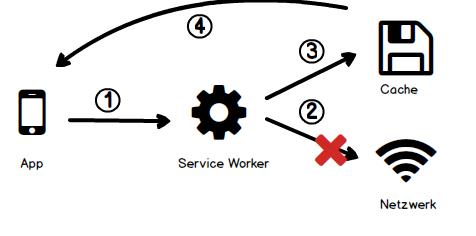
\includegraphics[width=0.75\textwidth]{networkfirst.png}
	\caption{\enquote{Erst Netzwerk, dann Cache}}
	\label{fig:cachingNetworkFirst}
\end{figure}



\subsubsection{\enquote{Erst Cache, dann Netzwerk}}
Wie Abbildung \ref{fig:cachingCacheFirst} zeigt, wird der Request hier zuerst an den Cache weitergeleitet. Befindet sich die angefragte Datei nicht im Cache, wird die Anfrage als \ac{HTTP}-Request an den Server weitergeleitet. Dies ist die bevorzugte Strategie für die meisten Requests in Offline-First Anwendungen.\autocite[Kapitel 05]{BookBuildingPWAs}.

\begin{figure}[h]
	\centering
	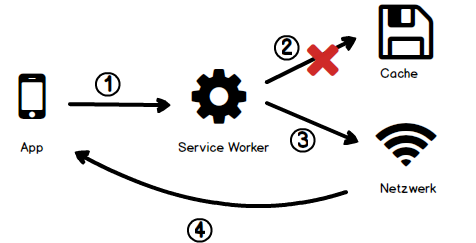
\includegraphics[width=0.75\textwidth]{cachefirst.png}
	\caption{\enquote{Erst Cache, dann Netzwerk}}
	\label{fig:cachingCacheFirst}
\end{figure}

\subsubsection{\enquote{Nur Netzwerk}}
Für Aufgaben, die nur online zu erfüllen sind, eignet sich die in Abbildung \ref{fig:cachingNetworkOnly} bezeichnete Strategie. Hier leitet der Service Worker den Request nur an das Netzwerk und nie an den Cache weiter. Offline-First Applikationen sollten so konzipiert sein, dass diese Art Requests im Falle einer unterbrochenen Internetverbindung nachgeholt werden können, wenn der Nutzer wieder online ist.

\begin{figure}[h]
	\centering
	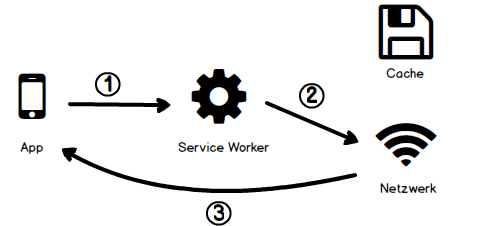
\includegraphics[width=0.75\textwidth]{networkonly.png}
	\caption{\enquote{Nur Netzwerk}}
	\label{fig:cachingNetworkOnly}
\end{figure}

\subsubsection{\enquote{Nur Cache}}
Abbildung \ref{fig:cachingCacheOnly} zeigt, wie die angefragte Ressource nur im Cache abgefragt wird. Diese Strategie ist nur dann sinnvoll, wenn die betroffenen Daten in einem vorherigen Schritt, beispielsweise beim Installieren des Service Workers, mit gecached wurden.

\begin{figure}[h]
	\centering
	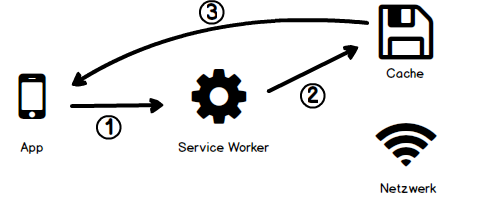
\includegraphics[width=0.75\textwidth]{cacheonly.png}
	\caption{\enquote{Nur Cache}}
	\label{fig:cachingCacheOnly}
\end{figure}

\section{Offline First Applikationen als verteilte Systeme}\label{sec:OfflineFirstVerteiteSysteme}
\citet{ArticleDistributedSystems} beschreiben verteilte Systeme wie folgt: \enquote{Ein verteiltes System ist eine Sammlung von autonomen Rechenelementen, die den Benutzern als ein einziges kohärentes System erscheint.}

Die folgende Liste zeigt die Charakteristika von verteilten Systemen, zusammengefasst nach \citet{BookDistributedSystemsDefinition}.

\begin{description}
\item[Eigenständige Computer] In einem verteilten System sind mehrere eigenständige Computer zu einem System verbunden. Diese können sich sowohl in der Hardware als auch in der Funktionsweise unterscheiden. 
\item[Singuläres Erscheinungsbild] Für den Nutzer sind die Unterschiede zwischen den einzelnen Computern im System unersichtlich. Er nimmt die verteilten Computer als ein einzelnes System wahr. 
\item[Konsistente und einheitliche Interaktion]
	Eine Konsequenz aus dem singulären Erscheinen ist, dass die Interaktion des Nutzers mit dem System immer gleich sein sollte, unabhängig davon, mit welcher Schnittstelle des Systems er tatsächlich interagiert. 
\item[Kontinuierliche Verfügbarkeit]
	Das System soll dem Nutzer kontinuierlich zur Verfügung stehen, auch wenn einzelne Teile des Systems vorübergehend ausgefallen oder nicht erreichbar sind.
\end{description}
\label{tab:charakteristikaDistributedSystem}

%TODO satz einfügen Kleppnmann vortrag.
Die folgende Liste zeigt, dass funktionsfähige Offline-First Applikationen die gleichen Charakteristika aufweisen und fasst zusammen, welche Rolle diese Merkmale in der Applikation spielen.

\begin{description}		
\item[Eigenständige Computer] Der Server und verschiedene Endgeräte bilden ein System. Sobald ein Endgerät die Applikation zwischenspeichert, ist sie als eigenständiger Computer im System aktiv. Als Endgerät qualifiziert sich jedes Gerät, welches einen kompatiblen Browser betreibt, weshalb die Endgeräte auch untereinander über unterschiedlichste Hardware verfügen können.
\item[Singuläres Erscheinungsbild]Die Kernfunktionalität von Offline-First Applikationen ist die Offlinefunktionalität. Offline interagiert der Nutzer nur mit seinem Endgerät, online werden die Daten gleich an den Server geschickt. Diese Unterschiede sind für den Nutzer jedoch nicht von Belang. \item[Konsistente und einheitliche Interaktion]
Unabhängig davon, welches Endgerät der Nutzer verwendet, sollen ihm früher oder später die Änderungen aller im System aktiven Geräte angezeigt werden. Der Nutzer muss sich zu keinem Zeitpunkt Gedanken darüber machen, aus welchen Computern das System besteht.
\item[Kontinuierliche Verfügbarkeit]
Ein weiterer Aspekt, welcher sich aus der verbindlichen Offlinefunktionalität ergibt, ist die kontinuierliche Verfügbarkeit. Der Nutzer kann seine Arbeit auch fortführen, wenn der Server nicht erreichbar ist. Durch SEC landen diese Änderungen früher oder später im System, wodurch die getrennte Verbindung zum Server keine Auswirkungen auf dessen Funktionsumfang hat. 
\end{description}
\label{tab:charakteristikaOfflineFirst}

Daraus ergibt sich, dass es sich bei Offline-First Webanwendungen um verteilte Systeme handelt. Diese Erkenntnis kann dabei helfen, Probleme von Offline-First Applikationen zu lösen. Bei Offline-First handelt es sich um ein relativ junges Konzept. Obwohl Progressive Web Apps mittlerweile häufig im Netz anzutreffen sind, erfüllt deren Offlinefunktionalität selten Offline-First Kriterien. Für Probleme wie die in Abschnitt \ref{sec:Problemfeld} beschriebene Synchronisation von Daten gibt es deshalb wenige beschriebene Lösungsansätze oder konkrete wissenschaftliche Arbeiten (siehe \ref{sec:VerwandteArbeiten}). Mit verteilten Systemen hingegen beschäftigt sich die Informatik bereits seit den 70er Jahren \autocite{Andrews1999FoundationsOM}. Lösungen, welche für die Herausforderungen von verteilten Systemen entwickelt wurden, kommen also auch für Offline-First Webapplikationen in Frage. Eine dieser Lösungen ist die Nutzung von optimistischen Replikationsverfahren. 

\section{Replikation}

Eine der wichtigsten Grundlagen verteilter Systeme ist die Replikation von Daten. Datenreplikation beschreibt das Verwalten mehrerer Datenspeicher, genannt Replikationen. Diese Replikationen halten die gleichen Daten, befinden sich jedoch auf unterschiedlichen Computern \autocite[S.42]{ArticleOptimisticReplication}. \citet{BookDistributedSystemsConceptsAndDesign} nennen drei Aspekte, zu denen Replikation in verteilten Systemen entscheidend beiträgt: Performancesteigerung, erhöhte Verfügbarkeit und Fehlertoleranz. Somit trägt diese Technik entscheidend dazu bei, sowohl kontinuierliche Verfügbarkeit als auch konsistente Interaktion, beschrieben in \ref{tab:charakteristikaDistributedSystem}, zu garantieren. Vom aus dem Netz nicht mehr wegzudenkenden Caching bis hin zu aufwendigeren Aufgaben wie Load-Balancing oder der Verarbeitung von DNS-Requests bietet das Internet zahlreiche Anwendungsfelder, in denen Replikation angewendet wird. 

\subsection{Pessimistische Replikation: Strong Consistency}

Traditionelle Strategien, um die Replikationen auf dem selben Stand zu halten, folgen dem Modell der \ac{SC}. \ac{SC} setzt voraus, dass alle Replikationen stets identisch sind, als gäbe es konstant nur eine singuläre Kopie der Daten. Wenn ein Update auf einer Replikation erfolgt, muss es direkt auf allen weiteren Replikationen übernommen werden. 

Es gibt ein weites Spektrum an Lösungen, um \ac{SC} zu gewährleisten. Diese reichen von {Update-Everywhere} Systemen, die einzelne Änderungen sofort auf allen Replikationen speichern \autocite{ThesisUpdateEverywhere} bis zu \enquote{primary copy} Lösungen \autocite[S.14]{BookPrimaryReplica}, welche Änderungen von einem primären Datenspeicher auf alle weiteren Replikationen verteilen. Gemeinsam haben diese Algorithmen die Tatsache, dass sie keinen Zugriff auf Replikationen gewähren, welche nicht auf dem aktuellsten Stand sind \autocite[S.43]{ArticleOptimisticReplication}. Für Offline-First Anwendungen kommt diese Art der Replikation nicht in Frage. Die Anforderung, dass die Verbindung zum Netzwerk stets unterbrochen sein kann (siehe \ref{sec:DefinitionOfflineFirst}), ist mit diesem Prinzip nicht vereinbar. Sobald eine Replikation vom Netzwerk getrennt ist, ist es unmöglich zu garantieren, dass sie auf dem aktuellsten Stand ist.


\subsection{Optimistische Replikation: Eventual Consistency}

Die optimistische Replikation, auch genannt \acf{EC}, ist ein alternatives Modell der Datenreplikation, welches den Replikationen erlaubt, voneinander abzuweichen.

Die Implementierung von optimistischer Replikation bietet sich somit als Lösung für Systeme an, welche besonderen Wert auf kontinuierliche Verfügbarkeit legen, wie Offline-First Applikationen (siehe Sektion \ref{sec:OfflineFirstVerteiteSysteme}). 

Bei der Verwendung von optimistischer Replikation sind Änderungen an Replikationen jederzeit gestattet, auch wenn diese nicht auf dem aktuellsten Stand sind, oder keine Verbindung zum Netzwerk haben. Nimmt der Nutzer eine Änderung vor, so wird diese auf seiner Replikation sofort umgesetzt. Im Hintergrund wartet die Applikation nun darauf, diese Änderung an die restlichen Computer des verteilten Systems weiterzugeben sowie selbst Änderungen entgegenzunehmen und zu verarbeiten \autocite[S.46]{ArticleOptimisticReplication}. Ziel ist es, wie beim Modell der Strong Consistency, Einheitlichkeit unter den Replikationen herzustellen. Das Modell der \ac{EC} setzt jedoch nicht voraus, dass diese Einheitlichkeit sofort erfolgen muss, sondern nur zu einem beliebigen späteren Zeitpunkt. 

Da die Computer im System parallel Änderungen vornehmen können, kann es vorkommen, dass mehrere Replikationen das gleiche Datenobjekt modifizieren. Im Allgemeinen werden die Modifikationen zu unterschiedlichen Ergebnissen führen. Ist dies der Fall, spricht man von einem Konflikt. Das Ziel, Konvergenz zwischen den Replikationen zu erlangen, kann nur erreicht werden, wenn aus allen im Konflikt stehenden Änderungen eine einheitliche Lösung entsteht.

Deshalb muss ein System, welches \ac{EC} implementiert, die Funktionalität aufweisen, Konflikte zu beheben. Problematisch dabei ist, dass die Replikationen nicht auf dem gleichen Stand sind, bis der Konflikt vollständig behoben ist, selbst nachdem sie ihre Änderungen untereinander ausgetauscht haben. Der Prozess der Konfliktbehandlung kann voraussetzen, auf die manuelle Konfliktlösung von Nutzern oder die Daten anderer Replikationen zu warten \autocite{ArticleEventualConsistencyConflicts}.

Gerade in Offline-First Anwendungen ist die Konfliktbehandlung eine große Herausforderung, wie in Abschnitt \ref{sec:Problemfeld} ausgeführt wird. Um diese Herausforderung zu bewältigen, bietet das Modell der \acf{SEC} einen Ansatz, die Flexibilität von \ac{EC} um die Sicherheit von \ac{SC} zu erweitern. 



%TODO: Nachteile Eventual Consistency:
%- Conflict Resolution
%- Garantiert nur, dass alle Updates ankommen. Dies kann zu Konflikten führen (Node A schreibt X=2, Node B schreibt X=3. Also ist erst A dann B = 3, erst B dann A = 2). Kann behoben werden durch Conflict Resolution, aber die ist stressig. 
%- Überleitung zu SEC. In SEC kommen alle Updates in der gleichen Reihenfolge, so kann komplexe Conflict Resolution umgangen Werden. 

\subsection{Strong Eventual Consistency}

%TODO Auf dem gleichen Stand = Konvergent/Konvergenz austauschen

\ac{SEC} beschreibt eine spezielle Form der \acf{EC}, welche das System von der Last der Konfliktbehandlung befreit. \ac{SEC} garantiert, dass zwei Replikationen nach dem Austauschen ihrer Änderungen immer konvergent sind. Im Gegensatz zur \ac{EC} wird die Konfliktbehandlung nicht vom System übernommen, stattdessen wird dieser Prozess durch die Nutzung spezieller Datentypen überflüssig. 

%TODO Abbildungen zu Consistencies
%TODO Evtl Charakteristika beschreiben 

\section{CRDTs}

CRDTs sind abstrakte Datentypen, die in verteilten Systemen eingesetzt werden, um \ac{SEC} zu ermöglichen. Sie basieren auf klassischen Datentypen wie Registern, Sets und Maps. CRDTs erweitern diese Datentypen um eine Schnittstelle, welche das Daten-Objekt neben den klassischen Operationen wie dem Auslesen des gespeicherten Wertes um zusätzliche Funktionalitäten erweitert, um \ac{SEC} zu gewährleisten.\autocite[S.1 ]{ArticleCRDTOverview}

Der Satz an CRDT-Funktionalitäten enthält immer eine Funktion zum Aktualisieren des Wertes des Objekts. Weitere Daten, um welche CRDTs klassische Datentypen erweitern, lassen sich als Metadaten beschreiben. Ihr Zweck ist es, die Aktualisierungs-Funktionalität möglich zu machen. Soll ein CRDT-Objekt beispielsweise so aktualisiert werden, dass sich die neueste Änderung des Wertes immer gegen ältere durchsetzt, muss zusätzlich zum Wert noch ein Zeitstempel der letzten Änderung verwaltet werden (siehe \ref{sec:LWW REGISTER}).
%todo WERT = Besseres wort finden? Value?
%todo: Abbildung CRDT mit Value, Merge, Zusatz
Die Datentypen werden speziell so modelliert, dass das Aktualisieren von CRDTs kommutativ, assoziativ und idempotent erfolgen kann \autocite{InproceedingsCrdtsInProduction}.

\begin{description}
	\item[Kommutativ] Wenn zwei CRDTs Aktualisierungen austauschen, ist das Ergebnis identisch, unabhängig davon, in welcher Reihenfolge dies geschieht.% (a merge b == b merge a)
	\item[Assoziativ] Wenn drei CRDTs nacheinander zusammengeführt werden, ist das Ergebnis immer gleich, unabhängig davon, welche zwei der Objekte zuerst Aktualisierungen austauschen.% (a merge (b merge c) == b merge (a merge c))
	\item[Idempotent] Das einmalige Zusammenführen zweier CRDTs hat das gleiche Ergebnis wie ein beliebig häufiges Wiederholen des Vorgangs.%(a merge b = ((((a merge b)merge b)merge b)merge b))
\end{description}

Diese Eigenschaften führen dazu, dass sich zwei Replikationen deterministisch im gleichen Zustand befinden müssen, sobald sie den Stand ihrer Daten synchronisiert haben. Im Gegensatz zur \ac{EC} ist das System nicht mehr von einer im Konsens zu geschehenden Konfliktlösung abhängig. 

Dieser Vorteil von \ac{SEC} ist gleichzeitig der größte Nachteil bei der Nutzung von CRDTs in der Praxis. Nicht alle Datenstrukturen lassen sich so modellieren, dass sie die benötigten oben genannten Anforderungen erfüllen. Zwar gibt es bereits viele, gut dokumentierte, kompatible Datentypen (siehe \ref{sec:Verwandte Arbeiten}), dennoch bedarf die Verwendung von CRDTs und \ac{SEC} ausgiebiger Planung und ist in manchen Fällen schlichtweg nicht möglich.

In der Literatur werden CRDTs in state-based und operation-based unterteilt \autocite[S. 10]{ArticleOptimisticReplication}. Die Unterscheidung erfolgt danach, wie das Zusammenführen der Objekte funktioniert.

\begin{description}
\label{sec:stateopbased}
	\item[State-based]
	Beim Synchronisieren von state-based CRDTs wird der gesamte Zustand der Objekte ausgetauscht.
	Die Merge-Funktion ist anschließend in der Lage, beide Zustände zu einem zu kombinieren. 
	
	\item[Operation-based]
	Bei der Variante der operation-based CRDTs wird nicht der gesamte State der Objekte ausgetauscht. Stattdessen erfolgt der Austausch über einzelne Updates. Wird der State eines Objektes geändert, so wird die Operation, welche die Änderung hervorgerufen hat, gespeichert. Beim Mergen zweier Objekte werden diese Updates ausgetauscht und anschließend auf das jeweils andere Objekt angewandt. Da die Operationen kommutativ sein müssen,
	%todo Siehe oben?
	ist die Reihenfolge der Updates nicht relevant. 
\end{description} 

Beide Kategorien sind äquivalent\autocite[S. 9]{InproceedingsCRDTOriginal}, was bedeutet, dass ein state-based CRDT ein operation-based CRDT emulieren kann und umgekehrt.

%todo hier ein paar beispiele oder so ka

\subsection{LWW-Register}
\sloppypar
Ein Register ist ein Objekt, welches einen einzelnen Wert verwaltet. Dieser Wert kann jede vom System unterstützte Datenstruktur sein. Ein \ac{LWW-Register} verfügt neben dem Wert noch über einen Zeitstempel. Wird der Wert des Registers geändert, wird auch der Zeitstempel auf den Zeitpunkt dieser Änderung gesetzt. Beim Zusammenführen zweier Register kann so immer die neuste Änderung übernommen werden. Da sowohl Wert als auch Zeitstempel ausgetauscht werden, handelt es sich hier um ein state-based CRDT.


%TODO Counter auslassen weil ich ihn nicht benutze?
\subsection{Grow-Only Set}
\label{sec:g-set}
Ein Set ist abstrakter Datentyp, welcher eine Sammlung von Objekten verwaltet. Traditionelle Operationen eines Sets umfassen das Hinzufügen und Entfernen von Objekten. Diese Operationen sind jedoch nicht kommutativ: Wird dem Set ein Objekt erst hinzugefügt und anschließend entfernt, ist es im Endeffekt nicht mehr im Set vorhanden. Wird es jedoch erst entfernt und anschließend hinzugefügt, so existiert das Objekt weiterhin im Set.

Ein Grow-Only Set löst dieses Problem durch das Auslassen der Entfernen-Operation. Das Entfernen des Objektes kann durch eine \enquote{Tombstone} Markierung ersetzt werden. Ist diese Markierung gesetzt, wird der Eintrag vom System so behandelt, als wäre er nicht vorhanden. Somit ist das Set wieder kommutativ, und die Funktionalität des Löschens bleibt bestehen. 

%todo OPERATIONEN KURSIV? IRGENDWIE HERVORHEBEN


\chapter{Konzeption}

\section{Idee des Prototypen}
Ziel der Arbeit ist es, einen Prototypen zu entwickeln welcher die Nutzung von CRDTs in Offline-First Webanwendungen demonstriert. Da die Datenstruktur hier im Mittelpunkt steht, liegt es nahe, als Prototyp eine Applikation zu entwickeln in der Nutzer auf verschiedenen Wegen mit Daten interagieren.

Deshalb wird eine Applikation zum Verwalten von Rezepten entwickelt, welche es Nutzern ermöglicht, ein gemeinsames Rezeptebuch zu pflegen. Da Nutzer in der Lage sein sollen online, offline und zur gleichen Zeit Rezepte anlegen, speichern und bearbeiten zu können, ist dies ein geeignetes Szenario um die Nutzung von CRDTs zu begutachten. 

\section{Anforderungsanalyse}
\label{sec:anforderungsanalyse}

In diesem Kapitel werden die funktionalen und nicht-funktionalen Anforderungen an den im Rahmen dieser Arbeit entwickelten Prototypen beschrieben.

\subsection{Funktionale Anforderungen}
Zweck der funktionalen Anforderungen ist es, Verhalten und Funktionalität zu entwickelnden Systems zu beschreiben. Die formulierten Anforderungen sollen somit einen Überblick darauf geben, was das implementierte System erfüllen muss. Da das Ziel dieser Arbeit die Entwicklung einer Datenstruktur für eine Offline-First Applikation ist (siehe \ref{sec:Einleitung}), liegt der Fokus der gesammelten Anforderungen eindeutig auf dem Zusammenspiel zwischen Offline-First und CRDTs.

Üblich in einer Anforderungsanalyse ist, die Anforderungen in \enquote{kann}, \enquote{soll} und \enquote{muss} Kategorien einzuteilen. Da es sich hier um die Entwicklung eines Prototypen handelt, wird sich in diesem Teil exklusiv auf \enquote{muss} Anforderungen beschränkt. Hierbei handelt es sich um Anforderungen, welche essentiell für das System sind.

\begin{description}
	\item[Anlegen von Rezepten]
	Nutzer sollen Rezepte anlegen können. Ein Rezept hat einen Namen und eine Liste an Zutaten. 
	\item[{[FA 1]} Anlegen von Zutaten]
	Die Nutzer sollen in der Lage sein, Zutaten zu einem Rezept hinzuzufügen. Zutaten haben einen Namen und eine Mengenangabe, welche die Nutzer setzten können.
	\item[Bearbeiten und Löschen]
	Den Nutzern soll es möglich sein, Rezepte und Zutaten zu bearbeiten und zu löschen. 
	\item[{[FA 2]} Zugriff mit mehreren Endgeräten gleichzeitig]
	Nutzer sollen in der Lage sein, mit mehreren Geräten gleichzeitig auf die gleiche Applikation zuzugreifen.
	\item[{[FA 3]} Offline-Erreichbarkeit]
	Nutzer der Anwendung müssen in der Lage sein, die Anwendung offline zu nutzen. Der Funktionsumfang der Applikation soll dadurch nicht beeinflusst werden. 
	\item[{[FA 4]} Lokales Speichern]
	Die Anwendung muss über die Funktionalität verfügen, Änderungen von Nutzern lokal zu speichern, damit diese auch zur Verfügung stehen wenn keine Verbindung zum Netzwerk besteht.
	\item[Online Speichern]
	Die Anwendungsdaten sollen nicht exklusiv lokal, sondern auch im Internet gespeichert werden können. Das Speichern der Daten erfolgt sinngemäß auf einem Server. 
	\item[{[FA 5]} Synchronisierung von Daten]
	Änderungen des Nutzers müssen mit dem Server synchronisiert werden können, wenn eine Verbindung zum Internet besteht. Der Nutzer sollte niemals seine offline umgesetzten Änderungen verlieren.
	\item[\ac{SEC}] Nachdem sich zwei Nutzer mit dem Stand des jeweils anderen Nutzers synchronisiert haben, müssen beide Applikationen den gleichen Stand haben.
	\item[{[FA 6] Konfliktfreies Synchronisieren}] Das Synchronisieren der Daten soll ohne Konflikte erfolgen. 
\end{description}


\subsection{Nicht-funktionale Anforderungen}
Während die funktionalen Anforderungen direkt Bezug auf die Funktionalität des Prototypen nehmen, werden zusätzlich sogenannte nicht-funktionale Anforderungen definiert, um die Rahmenbedingungen des Projekts einzuschränken. Diese beziehen sich nicht auf die konkreten Funktionen, sondern beschreiben stattdessen Ziele, welche die Umsetzung des Prototypen über die Funktionalität hinaus hat. 

\begin{description}
	\item[{[NFA 1]} Anschauliche Umsetzung: Code]
	Ein Ziel der Arbeit ist, zu ermitteln, wie CRDTs in modernen Webanwendungen umgesetzt werden können (siehe \ref{sec:Problemfeld}). Da sich moderne Offline-First Anwendungen leider nicht in auf ein einziges Beispiel reduzieren lassen, ist bei der Umsetzung darauf zu achten die Datenstruktur so anschaulich und verständlich wie möglich zu implementieren. Dies bedeutet beispielsweise, Lesbarkeit über Effizienz beim schreiben von Programmcode zu priorisieren.
	\item[{[NFA 2]} Anschauliche Umsetzung: Technologien]
	Um das in NFA 1 formulierte Ziel der Anschaulichkeit weiter zu verfolgen, soll auch die Wahl der Technologien so erfolgen, dass diese soll die Ebene der Datenstruktur in Javascript umgesetzt werden. Auch wenn Entwicklern heutzutage zahlreiche Sprachen zur Verfügung stehen, welche zu Javascript kompilieren, bleibt Javascript aufgrund der hohen Verbreitung die für demonstrative Zwecke geeignetste Sprache.
	\item[{[NFA 3]} Unabhängigkeit von Datenbank-Technologien]
	Die implementierte Datenstruktur muss unabhängig von der benutzten Datenbank sein. Keine der umgesetzten CRDT-Funktionalitäten darf von der gewählten Datenbank abhängig sein.
\end{description}

\section{Architektur}
\label{sec:Architektur}

Da Daten sowohl online als auch offline gespeichert werden sollen, folgt die Umsetzung der Applikation dem für Webseiten üblichen Client-Server Modell. 

Das der Prototyp als Offline-First Anwendung umgesetzt wird und umfangreiche Offlinefunktionalität zentraler Bestandteil der funktionalen Anforderungen sind, wirkt sich entscheidend auf die Architektur aus.

Die Nutzung eines Service-Workers (siehe \ref{sec:serviceworker}) ermöglicht das zwischenspeichern der gesamten Client-seitigen Dateien, welche zum ausführen der Applikation benötigt werden. Da die Speicherung der Anwendungsdaten auch lokal erfolgen soll, ist die Anwendung nicht darauf angewiesen bei jeder Aktion des Nutzers Daten an den Server zu schicken.

\begin{figure}[h]
	\centering
	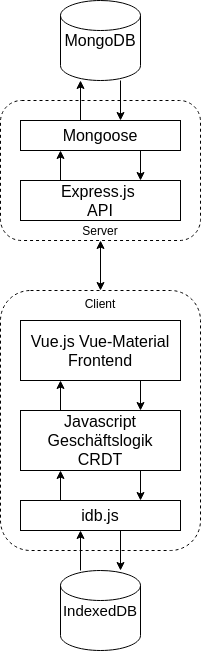
\includegraphics[width=0.25\textwidth]{architektur.png}
	\caption{\enquote{Architektur des Prototypen}}
	\label{fig:architektur}
\end{figure}

Abbildung \ref{fig:architektur} zeigt die Architektur des Prototypen. Die Clientseite setzt sich zusammen aus Frontend, Geschäftslogik und der Browser-API IndexedDB als lokalen Speicher. Zusätzlich wird die JavaScript library \enquote(idb.js) für den Zugriff auf IndexedDB genutzt. Die CRDT Funktionalitäten befinden sich in dieser Darstellung in der Geschäftslogik. 

Die Serverseite beginnt mit einer API, welche nur eine einzelne \enquote{/sync} Route zur Synchronisierung von lokalen- und online-Daten bereitstellt. Über diese Schnittstelle kann der Client seine Operationen an den Server schicken und erhält als Antwort die gesammelten Operationen des Servers. Das server-seitige Speichern der Applikationen erfolgt auf einer MongoDB Datenbank. Ergänzend zu MongoDB wird noch die library Mongoose genutzt. Als Laufzeitumgebung zum Betreiben des Webservers dient Node.js.

\section{Technologien}

Es folgt eine kompakte Vorstellung der zur Umsetzung des Prototypen genutzten Technologien. Auch wird erläutert, warum die einzelnen Technologien verwendet werden.

\subsection{JavaScript, HTML und CSS}
JavaScript ist eine Skriptsprache welche zur clientseitigen Programmierung von Websites genutzt wird. Mit einer Nutzung in über 95\% \autocite{OnlineJavascriptDistr} aller Websites ist sie aus dem Internet nicht wegzudenken. In den letzten Jahren gewannen auch Sprachen an Popularität, die zu JavaScript kompilieren, wie zum Beispiel TypeScript oder ClojureScript. Da JavaScript die Basis dieser Sprachen bildet und sich gut in diese Übersetzten lässt, ist eine Implementierung in der \enquote{Grundsprache} am besten dazu geeignet, die Anforderung eine anschaulichen und verständlichen Umsetzung zu erfüllen.
\subsection{VueJS}
Da es sich beim Prototypen nicht um eine statische Website handelt, sondern oft Änderungen an der Nutzeroberfläche oder an den Applikationsdaten vorgenommen werden, bietet sich die Nutzung eines Frameworks, welches diese Interaktionen vereinfacht, an. 

VueJS ist ein JavaScript Framework zum Erstellen von Benutzeroberflächen. Die Nutzung von VueJS erlaubt die Verknüpfung von HTML-Elementen mit Anwendungsdaten. So können HTML-Elemente automatisch aktualisiert werden, wenn sich ein Wert in einem Vue-Objekt ändert. Diese Verknüpfung macht auch Änderungen in die Umgekehrte Richtung möglich, also die Aktualisierung von Applikationsdaten bei Änderungen welche auf Seite der Nutzeroberfläche gemacht werden.

Ein Feature von VueJS ist die Erzeugung von \enquote{components}. Hierbei handelt es sich um VueJS Instanzen, welche in HTML wiederverwendet werden können. Bei der Umsetzung des Prototypen wird die component-library vue-material genutzt, um Zugriff auf einige vorgefertigte Komponenten wie Buttons und Eingabefelder zu haben. 
\subsection{IndexedDB}
IndexedDB ist eine Browser-API welche das clientseitige Speichern von Daten im Browser ermöglicht. Das bedeutet, dass über IndexedDB gespeicherte Daten auch offline zur Verfügung stehen. Die Nutzung der IndexedDB Schnittstelle bietet dem Prototypen die Funktionalität der Speicherung von Offline-Daten, welche für die Erfüllung der funktionalen Anforderungen rund um Offline-First-Eigenschaften essenziell ist. 

Über sogenannte ObjectStores können JavaScript Objekte gespeichert und ausgelesen werden. Die Abfrage der Objekte erfolgt über einen der Werte des Objekts, welcher als Schlüssel konfiguriert wird. Alle Änderungen welche an der Datenbank vorgenommen werden, erfolgen in Transaktionen. Änderungen an der Datenbank bestehen nur, wenn eine Transaktion erfolgreich war. Bei Komplikationen wird die Transaktion abgebrochen, wodurch die an der Datenbank während der Transaktion vorgenommenen Änderungen rückgängig gemacht werden. Somit bieten Transaktionen einen gewissen Schutz von Anwendungs- und Systemfehlern. Dies ist ein wichtiger Aspekt für die fehlerfreie Gewährleistung der CRDT-Funktionalitäten.
\subsection{idb}
Die Event- und Callback-basierte Schnittstelle, welche IndexedDB bietet, führt dazu, dass sehr komplexer Code geschrieben werden muss um simple Operationen an der Datenbank durchzuführen \autocite{InproceedingsIDBdoof}. Um dieses Problem zu vermeiden und guten, lesbaren Code zu schreiben wird bei der Umsetzung des Prototypen auf die library idb zurückgegriffen. Bei idb handelt es sich um einen API-Wrapper, welche die API vereinfacht und Zugriff auf die Datenbank über JavaScript Promises anstelle von Events und Callbacks bietet. Listing \ref{lst:indexeddbexample} zeigt das erzeugen eines Object-Stores über die gewöhnliche IndexedDB API, in Listing \ref{lst:idbexample} ist die gleiche Aktion mit der idb API umgesetzt. Während in der gewöhnlichen Variante mit Callbacks weitergearbeitet werden muss, gibt die idb API mit \enquote{idb.open} ein Promise zurück.

\begin{minipage}{\linewidth}
\lstinputlisting[language=JavaScript, caption=IndexedDB: öffnen eines Object-Stores, label={lst:indexeddbexample}]{code/indexedexample.js}
\end{minipage}

\begin{minipage}{\linewidth}
\lstinputlisting[language=JavaScript, caption={idb: öffnen eines Object-Stores}, label={lst:idbexample}]{code/idbexample.js}
\end{minipage}

\subsection{Node.js, Express.js, MongoDB}

Obwohl die entwickelte CRDT Implementierung mit jeder Datenbank kompatibel ist, die Daten schreiben, lesen und suchen kann, wird zu demonstrativen Zwecken doch ein Node.js Server aufgesetzt der mit einer MongoDB Datenbank verbunden ist. Node.js ist eine JavaScript Laufzeitumgebung, welche gewöhnlich zum Betreiben von Webservern genutzt wird. Für das Bereitstellen der einzelnen Route wird, wie üblich, Express.js genutzt. Die Datenbank muss, wie in Sektion \ref{sec:Architektur} erläutert, nur eine Tabelle für das Speichern von Operationen verwalten. Als Beispiel wird hier eine MongoDB Datenbank mit Mongoose als Object Data Modeling library verwendet. Die Wahl fiel auf MongoDB weil es eine populäre Datenbank ist, funktionale Kriterien spielten bei der Wahl der Datenbank keine Rolle. 

\subsection{Sonstiges}
UUIDv4, google Roboto font, google material icons

\section{Entwurf der Nutzeroberfläche}

Aus den funktionalen Anforderungen lässt sich ein Entwurf für die Nutzeroberfläche des Prototypen erstellen. Abbildung \ref{fig:rezepteFrame} zeigt den Hauptbildschirm der Website. Hier kann der Nutzer Rezepte hinzufügen, löschen und die Namen der angelegten Rezepte bearbeiten. Der \enquote{Sync} Button initialisiert das Synchronisieren mit dem Server. Über den Knopf \enquote{Zutaten} gelangt der Nutzer zur Übersicht der Zutaten des jeweiligen Rezepts. Wie auf Abbildung \ref{fig:zutatenFrame} zu erkennen ist, kann der Nutzer hier neue Zutaten für das Rezept anlegen und bestehende Zutaten bearbeiten oder löschen. Darüber hinaus kann er jeder angelegten zutat eine Menge zuweisen, und auch diese bearbeiten. 

\begin{figure}[h!]
	\centering
	\begin{minipage}{.45\textwidth}
		\centering
		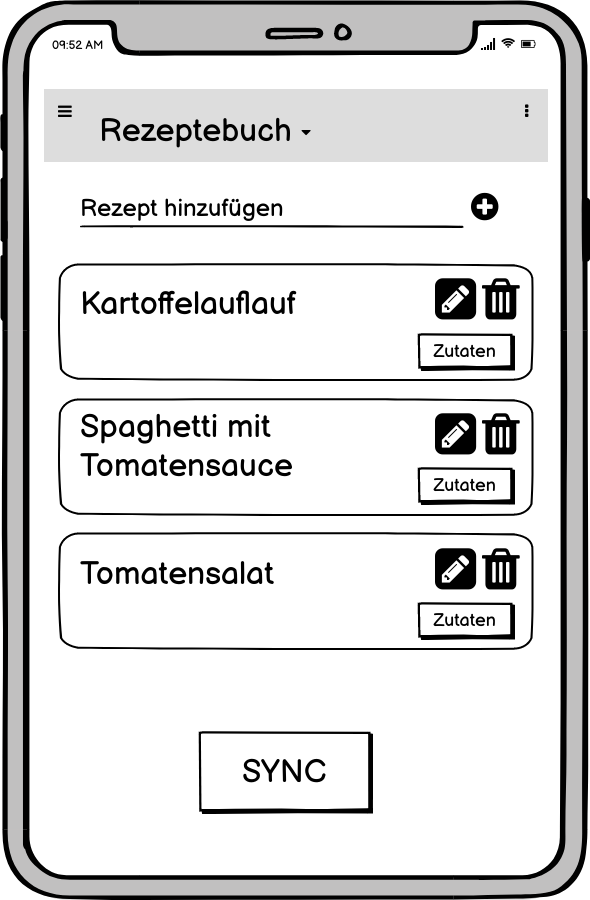
\includegraphics[width=1\textwidth]{wireframeRezepte2.png}
		\caption{\enquote{Hauptbildschirm}}
		\label{fig:rezepteFrame}
	\end{minipage}
	\begin{minipage}{.45\textwidth}
		\centering
		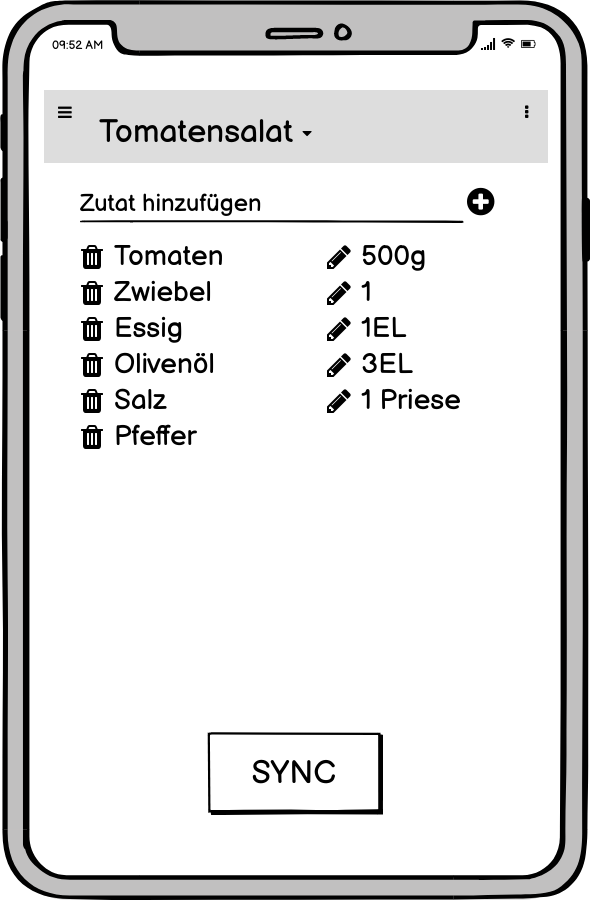
\includegraphics[width=1\textwidth]{wireframeZutaten2.png}
		\caption{\enquote{Übersicht Zutaten}}
		\label{fig:zutatenFrame}
	\end{minipage}
\end{figure}



\section{Datenstruktur}

Diese Sektion beschreibt die Planung der Datenstruktur für den Prototypen. Erster Schritt dieser Planung ist es, zu ermittelt, welche Daten von der Datenstruktur verwaltet werden müssen und wie diese von der Applikation genutzt werden. Das Vorgehen ist, die Grundlagen der Datenstruktur erst in konventionellen Datentypen zu entwerfen und diese anschließend um CRDT Funktionalitäten zu erweitern. Dies bietet sich an da, CRDTs üblicherweise auf konventionellen Datentypen aufbauen und die Datenstruktur schließlich auf die Applikation zugeschnitten sein soll und nicht umgekehrt. Würde mit dem Entwurf des CRDT begonnen werden, bevor die Grundlagen der Applikation festgelegt sind, müsste sich die Applikation der Datenstruktur anpassen. Dies gilt es zu vermeiden, es sei denn die Rahmenbedingungen fordern aus anderen Gründen eine bestimmte Datenstruktur, was in dieser Arbeit jedoch explizit nicht der Fall ist. Ziel des Prototypen ist es, die Datenstruktur an die Applikation anzupassen. 

\subsection{Grundlagen der Datenstruktur}

Die in Sektion \ref{sec:anforderungsanalyse} formulierten Anforderungen formulieren, dass es in der Applikation um das Speichern, bearbeiten und Löschen von Rezepten und ihren Zutaten geht. Nun gilt es, zu modellieren, wie ein solches Rezept als Objekt in der Applikation aussieht. 

Listing \ref{lst:rezeptv1} zeigt die die Struktur eines Rezeptes als einzelnes JavaScript Objekt. Neben einer ID verfügt es noch über die Eigenschaften \enquote{name}, welche den Namen des Rezepts speichert und die Eigenschaft \enquote{ingredients}. Bei \enquote{ingredients} handelt es sich um ein Array an Objekten, welche jeweils eine Zutat mit Namen (\enquote{name}) und Mengenangabe (\enquote{measure}) abbilden. Darüber hinaus erhält das Rezept zur Identifikation eine generierte ID. Da, wie in Sektion \ref{fig:architektur} erläutert, das lokale Speichern über die IndexedDB API erfolgt, können die Rezepte auch direkt als Objekte in der Datenbank des Browsers gespeichert werden. Auch die Verschachtelung der Objekte stellt kein Problem dar, da IndexedDB auch Objekte mit Objekten als Eigenschaft speichert. Zwischen Applikation und lokalem Speichern muss folglich keine Umwandlung der Daten erfolgen.

%In diesem Modell ist ein Rezept schlussendlich ein verschachteltes Objekt und die gesamten Applikationsdaten lassen sich in einer Sammlung aller Rezepte finden. Übertragen auf abstrakte Datentypen wäre ein Rezept eine Map. Diese Map enthält die Schlüssel \enquote{name} und \enquote{ingredients}. Während zu dem Schlüssel \enquote{name} ein String als Wert gespeichert werden soll, dient der Schlüssel \enquote{ingredients} zur Speicherung der Zutaten des Rezeptes. Da ein Rezept mehr als eine Zutat haben kann, handelt es sich hierbei um ein Set. Dieses Set besteht wiederum aus den Zutaten Objekten, welche, genau wie das Rezept, Daten in Schlüssel-Wert Paaren beinhalten. Somit handelt es auch bei den Zutaten um Maps.

%Somit wäre ein Rezept schlussgefolgert eine Map, welche einen einzelnen Wert und ein Set speichert, welches wiederum eine unbestimmte Anzahl an Maps speichert, welche wiederum einzelne Werte speichern.

\begin{minipage}{\linewidth}
	\lstinputlisting[language=JavaScript, caption={Beispiel Rezept verschachtelt}, label={lst:rezeptv1}]{code/recipev1.js}
\end{minipage} 

Ein solches Modell ist nicht unüblich und gerade in JavaScript Anwendungen, weil Objekte in diesen oft verschachtelt sind, häufig praktisch. Beim Einsatz von CRDTs jedoch, lohnt es sich die Datenstruktur so flach wie möglich zu gestalten. Wir erinnern uns -- Ein CRDT baut auf normalen Datenstrukturen auf. Wenn es die Möglichkeit gibt, die Komplexität der ausgehenden Datenstruktur zu reduzieren, bedeutet dass auch eine Reduzierung an Komplexität für die zu implementierenden CRDT-Funktionalitäten.

Eine Option, die Datenstruktur abzuflachen besteht darin, die in Listing \ref{lst:rezeptv1} gezeigten Daten zu normalisieren und somit relational abzubilden. In diesem Fall werden die Zutaten nicht als Array in dem Rezept verschachtelt, sondern werden einzeln gespeichert. Listing \ref{lst:rezeptv2} zeigt ein Rezept in der relationalen Modellierung, Listing \ref{lst:ingredientv2} eine dazugehörige Zutat. Die Verbindung zwischen Rezepten und Zutaten wird nun über die Eingenschaft \enquote{recipe} der Zutaten definiert. Hier wird die ID des Rezepts hinterlegt, welchem die Zutat zugehörig ist.

%TODO NORMALISIERUNG DARSTELLEN

\begin{minipage}{\linewidth}
	\lstinputlisting[language=JavaScript, caption={Beispiel Rezept relational}, label={lst:rezeptv2}]{code/recipev2.js}
\end{minipage}

\begin{minipage}{\linewidth}
\lstinputlisting[language=JavaScript, caption={Beispiel Zutat relational}, label={lst:ingredientv2}]{code/ingredientsv2.js}
\end{minipage}

\subsection{Erweiterung zum CRDT}

Währen sich bei konventionellen Datentypen nicht viel daran ändert, ob eine Zutat über \enquote{recipe.ingredient}, wie es in Listing \ref{lst:rezeptv1} der Fall wäre, oder \enquote{ingredient}, siehe Listing \ref{lst:rezeptv2} angesprochen wird, wäre die Umsetzung als CRDT in der verschachtelten Variante deutlich komplexer. Die Ursache dafür ist, dass die Änderungen an Zutaten schließlich auch von CRDT-Funktionalitäten profitieren sollten. Das Modell für ein Rezept müsste deshalb als CRDT entworfen werden, welches ein weiteres CRDT als Eigenschaft hält. Dies ist in der Umsetzung durchaus möglich, in diesem Fall aber leicht durch die relationale Herangehensweise zu vermeiden.

Da in der Applikation kein universell einsetzbares CRDT entworfen werden soll, sondern eines was den Anforderungen der Anwendung gerecht wird, gilt es nun zu ermitteln, welche Schnittstellen es der Applikation zur Verfügung stellen muss. Aus der Anforderungsanalyse, welche in in Sektion \ref{sec:anforderungsanalyse} durchgeführt wurde, lassen sich die Anforderungen an das CRDT ableiten. Tabelle \ref{tab:crdtAnforderungen} fasst diese als Schnittstellen zusammen, welche die Datenstruktur der Applikation bereitstellen muss. 

\begin{table}[]
	\caption{CRDT Schnittstellen}
	\label{tab:crdtAnforderungen}
	\resizebox{\textwidth}{!}{%
		\bgroup
		\def\arraystretch{1,5}%
		\begin{tabular}{|l|l|}
			\hline
			\rowcolor[HTML]{EFEFEF} 
			Funktionale Anforderung & Datenstruktur Anforderung \\ \hline
			Anlegen von Rezepten & \begin{tabular}[c]{@{}l@{}}Verwaltung einer Sammlung von beliebig vielen Rezepten\\ Hinzufügen eines Rezepts in die Rezeptesammlung.\end{tabular} \\ \hline
			Anlegen von Zutaten & \begin{tabular}[c]{@{}l@{}}Verwaltung einer Sammlung von  beliebig vielen Zutaten\\ Hinzufügen einer Zutat in die Zutatensammlung.\end{tabular} \\ \hline
			Bearbeiten und Löschen & \begin{tabular}[c]{@{}l@{}}Bearbeitung der Eigenschaften Rezeptname, Zutatenname, Zutatenmenge.\\ Entfernen eines Rezeptes aus der Rezeptesammlung.\\ Entfernen einer Zutat aus der Zutatensammlung.\end{tabular} \\ \hline
		\end{tabular}%
		\egroup
	}
\end{table}

Die Umsetzung im Prototypen erfolgt durch ein \enquote{Operation-based} CRDT. Wie in Sektion \ref{sec:stateopbased} erläutert, werden alle Änderungen, welche an den Applikationsdaten erfolgen, einzeln als sogenannte Operationen abgespeichert. Wie Rezepte und Zutaten werden auch die Operationen über die IndexedDB API lokal im Browser gespeichert.

Listing \ref{lst:operationv1} zeigt eine Operation, welche beim Umbenennen des in Listing \ref{lst:rezeptv2} entworfenen Rezeptes erzeugt und gespeichert wird. Die Felder \enquote{store}, \enquote{object} und  \enquote{key} dienen der Identifikation des Wertes, der geändert werden soll, \enquote{value} beschreibt den neuen Wert. Die dargestellte Operation dokumentiert also, dass im Object-Store \enquote{recipes} der Wert des Schlüssels \enquote{name} vom Objekt \enquote{re\_ckdiw1bxw002411w66m7mol85s} zu \enquote{Tomaten-Paprika-Salat} geändert werden soll. Darüber hinaus erhält die Operation noch eine eigene ID und einen Zeitstempel. Der Zeitstempel dient dazu, eine konfliktfreie Synchronisation zu gewährleisten, mehr dazu im nächsten Abschnitt. 

\begin{minipage}{\linewidth}
	\lstinputlisting[language=JavaScript, caption={Beispiel Operation}, label={lst:operationv1}]{code/operationv1.js}
\end{minipage}

\subsection{Parallele Änderungen}

Zwei Replikationen können sich synchronisieren, indem sie ihre gespeicherten Operationen austauschen. Nachdem eine Replikation über diesen Weg eingehende Operationen erhalten hat, müssen die Operationen auf die Applikationsdaten angewendet werden, damit die Änderungen einen Effekt haben. Nachdem eine eingehende Operation angewandt wurde, wird sie zu den lokalen Operationen abgespeichert.

Beim Anwenden der Operationen kann es vorkommen, dass zwei Operationen Änderungen am gleichen Wert vorgenommen haben. Für solche Fälle, genannt parallele Änderungen, müssen Regeln implementiert werden, um zu entscheiden, welche der parallelen Änderungen den Vorzug bekommt. Nur so ist gewährleistet, dass zwei Replikationen nach dem Synchronisieren auf dem gleichen Stand sind, wäre die Auswahl zufällig, oder würde sich stets die lokale Änderung durchsetzen, könnten die Applikationsdaten von einander abweichen. So wäre Konvergenz zwischen den Replikationen und somit \ac{SEC} nicht gewährleistet und der Einsatz von CRDTs überflüssig.

Im Prototypen werden parallele Änderungen mit \ac{LWW} Regeln behandelt. Abbildung \ref{fig:flwochartOperationen} zeigt, wie entschieden wird, ob eine eingehende Operation angewendet wird. Zuerst wird überprüft, ob es für eine eingehende Operation, welche angewandt werden soll, bereits eine lokale Operationen gibt, welche den selben Wert betreffen. Ist dies der Fall, werden die Zeitstempel der aktuellsten lokalen Operation und der eingehenden Operationen verglichen. Ist die lokale Operation neuer als die eingehende Operation, wird die eingehende Operation ignoriert. Ist hingegen die eingehende Operation neuer, wird sie angewandt und anschließend, wie vorgesehen, zu den lokalen Operationen hinzugefügt.

\begin{figure}[H]
	\centering
	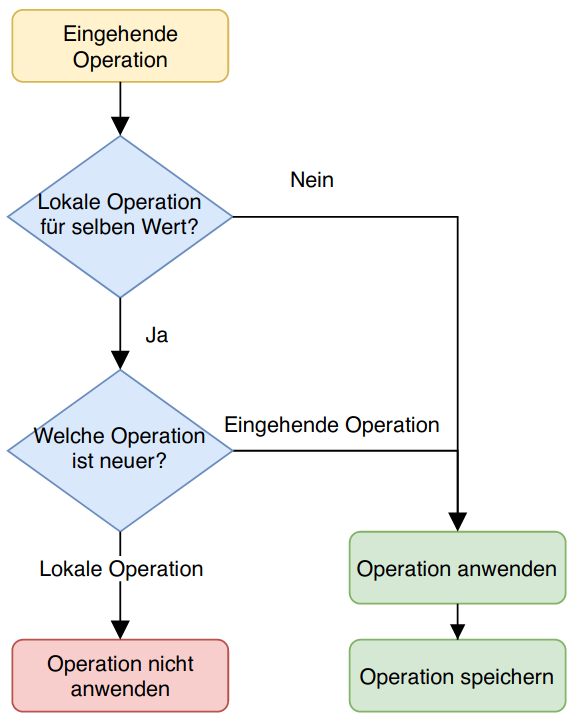
\includegraphics[width=0.6\textwidth]{flowchartOperationen.png}
	\caption{\enquote{Bearbeiten einer eingehenden Operation}}
	\label{fig:flwochartOperationen}
\end{figure}

\subsection{Anwenden von Operationen}

Auch beim Anwenden von Operationen gilt es, einigen potentiellen Fehlern aus dem Weg zu Gehen. Da die Operationen kommutativ anwendbar sein sollen, kann es vorkommen, dass ein Objekt bearbeitet werden soll, welches lokal noch nicht existiert. Damit eine solche Änderung nicht verloren geht, wird das Objekt beim Anwenden der Änderung erstellt, sollte es noch nicht existieren. Wichtig hierbei ist, dass das neue Objekt keine zufällige ID zugewiesen bekommt, sondern die in der Operation hinterlegte ID des fehlenden Objektes. Anschließend kann die Operation wie vorgesehen auf das neue Objekt angewandt werden. Durch diese Semantik ist es möglich, die \enquote{Erstellen} und \enquote{Bearbeiten} Schnittstellen (siehe Tabelle \ref{tab:crdtAnforderungen}) mit der gleichen Methode umzusetzen. Eine Operation zum Erstellen eines Objektes wird einfach genau wie eine Operation zum Bearbeiten angelegt, statt einer bestehenden ID beim Bearbeiten wird jedoch eine neue ID erzeugt. Somit wird das Objekt beim Anwenden der Operation erzeugt, da es sich um eine unbekannte ID handelt. 

Ein weiterer Fehlerfall droht beim Entfernen von Rezepten und Zutaten, welches neben dem Anlegen und Bearbeiten auch eine weitere Schnittstellen zur Datenstruktur ist (siehe Tabelle \ref{tab:crdtAnforderungen}). Abbildung \ref{fig:rezeptLöschenSchlecht} zeigt die Problematik, welche auftritt wenn das Objekt tatsächlich aus der Datenbank gelöscht wird. Wird ein Objekt gelöscht und anschließend bearbeitet kommt die Applikation nicht auf den gleichen Stand wie wenn die Operationen in umgekehrter Reihenfolge angewandt werden. Somit wäre erneut das Kommutativgesetz verletzt und die Applikationsdaten könnten sich nach dem Synchronisieren unterscheiden. 

\begin{figure}[H]
	\centering
	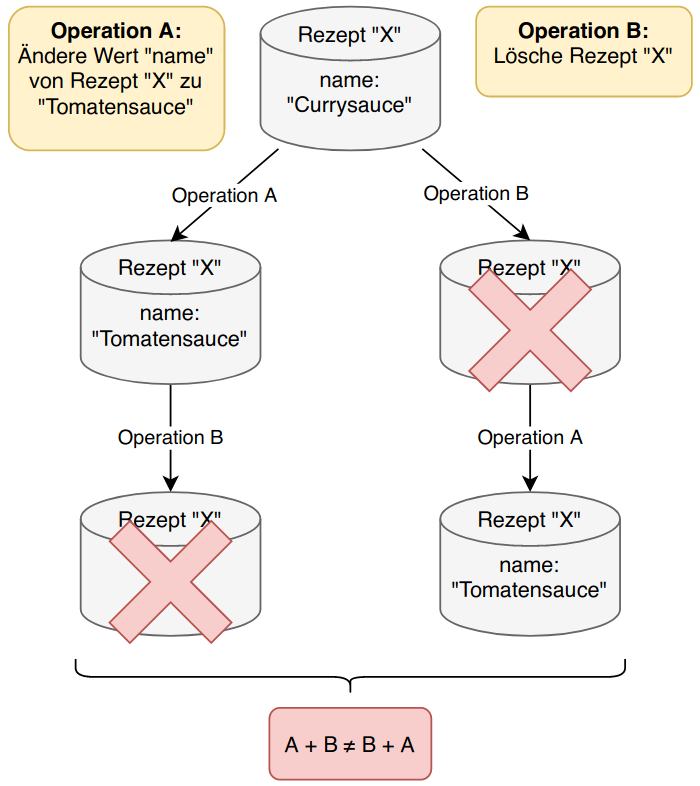
\includegraphics[width=0.66\textwidth]{deleteRecipeBad.png}
	\caption{\enquote{Fehlerfall beim Entfernen eines Rezeptes}}
	\label{fig:rezeptLöschenSchlecht}
\end{figure}

Im Prototyp werden die Rezepte- und Zutatensammlungen deshalb als G-Set (siehe Sektion \ref{sec:g-set}) implementiert. Dies bedeutet, dass Rezepte und Zutaten nicht mehr gelöscht werden können, nachdem sie einmal angelegt wurden. Stattdessen wird das Entfernen der Objekte über eine weitere Eigenschaft gelöst, den sogenannten \enquote{tombstone}. Beim \enquote{tombstone}, Englisch für Grabstein, handelt es sich um einen Statusindikator, welcher bestimmt ob ein Objekt von der Applikation als aktiv oder inaktiv behandelt werden soll. Somit kann auch das Entfernen eines Objektes auf die gleiche Herangehensweise erfolgen, wie das Anlegen und Bearbeiten.

\begin{minipage}{\linewidth}
	\lstinputlisting[language=JavaScript, caption={Beispiel Entfernen-Operation}, label={lst:operationv2}]{code/operationTombstone.js}
\end{minipage}

Listing \ref{lst:operationv2} zeigt, wie eine Entfernen-Operation ebenso Informationen über das Zielobjekt enthält. Der Angesprochene Schlüssel ist dabei immer \enquote{tombstone}, der Wert \enquote{1} indiziert, dass das Objekt als entfernt zu behandeln ist. Wäre eine Schnittstelle zum Reaktivieren des Objekts gewünscht, so könnte dies durch das ändern des \enquote{tombstone} Werts auf \enquote{0} umgesetzt werden. Abbildung \ref{fig:rezeptLöschenGut} zeigt, wie die Anwendung der vorher fehlerverursachenden Operationen durch die Nutzung des \enquote{tombstone} Indikators wieder Kommutativ ist.

\begin{figure}[H]
	\centering
	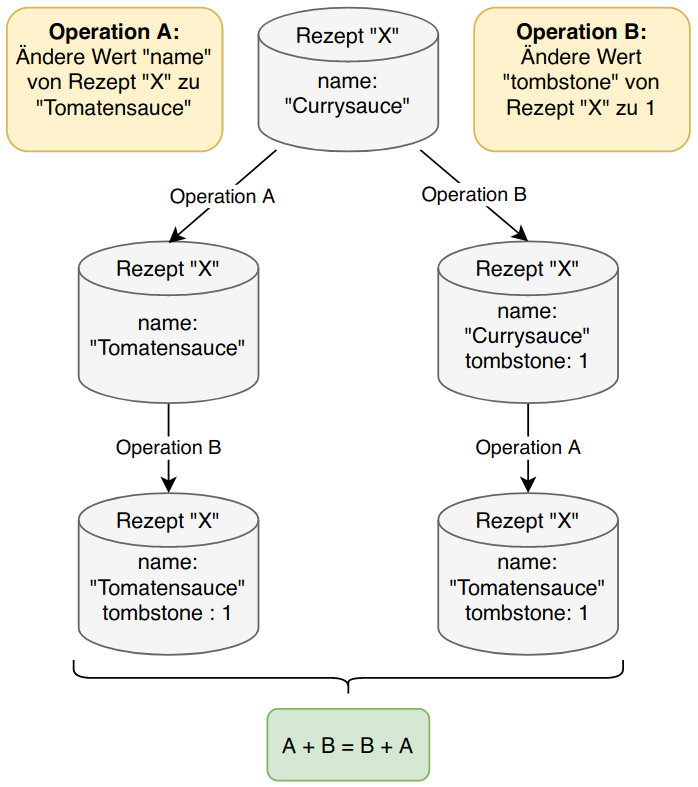
\includegraphics[width=0.66\textwidth]{deleteRecipeGood.png}
	\caption{\enquote{Korrektes Entfernen eines Rezeptes}}
	\label{fig:rezeptLöschenGut}
\end{figure}

\section{Server}

Diese Sektion beschreibt, wie der Server in der Architektur genutzt wird, um für das Verteilen von Operationen zu sorgen.

\subsection{API}

\subsection{Datenbank}

\section{Schnittstellen}
\newpage
\printbibliography



\end{document}]


